\documentclass[12pt]{article}
\usepackage[utf8]{inputenc}
\usepackage{amsmath}
\usepackage[document]{ragged2e}
\usepackage{graphicx}
\usepackage{xcolor}
\usepackage{caption}
\usepackage{float}
\usepackage{subcaption}

\title{SOP Fysikkformler}
\author{Magnus Trandokken}
\date{Høst 2022}

\setcounter{secnumdepth}{0}
\begin{document}

\centering
\pagenumbering{gobble}
\maketitle

\newpage
\pagenumbering{arabic}
\RaggedRight
\tableofcontents
\newpage

\section{Bevegelseslære}
\subsection{Rettlinjet bevegelse}
Def. av aksjelerasjon: $a = \frac{d\Vec{v}}{dt}$

\subsubsection{Bevegelsesformler}
\begin{enumerate}
    \item $v = v_0+at$
    \item $s = \frac{1}{2}(v+v_0)t$
    \item $s = v_0t+\frac{1}{2}at^2$
    \item $v^2 = v_0^2+2as$
\end{enumerate}
\section{Newtons Lover}
\begin{enumerate}
    \item $\sum{\Vec{F}} = 0 \Leftrightarrow \textbf{konstant akselerasjon }$
    \item $\sum{\Vec{F}} = m\Vec{a} \Rightarrow \Vec{a} || \Vec{F}$
    \item $\Vec{F}_{AB} = \Vec{F}_{BA}$ \textbf{Kraft = Motkraft!}
\end{enumerate}
\subsection{Fjærkrefter}
\textbf{Hooks lov: }\\ $\Vec{F}_{\text{fjær}} = -k\Vec{x}$\\
$k =$ fjærstivhet\\ $x =$ forlengelse/sammentrekning

\subsection{Friksjonskrefter}
\subsubsection{Hvilefriksjon}
$f_{s max} \leq \mu_sN = \mu_smg$, $\mu_s =$ hvilefriksjonskoeffisienten
\subsubsection{Glidefriksjon}
$f_k = \mu_kN = \mu_kmg$, $\mu_k =$ glidefriksjonskoeffisienten
%
%
\section{Sirkelbevegelse}
\begin{itemize}
    \item[] \textbf{Buelengde: } $S = \phi \cdot r$ (Radianer per sekund)
    \item[] \textbf{Buelengde av hel runde:} $S = 2\pi r$
    \
\end{itemize}

\subsection{Konstant banefart}
\begin{itemize}
    \item[] \textbf{Rotert vinkel}: $\theta$
    \item[] \textbf{Vinkelfart ($\omega$)}: $\frac{rad}{s} = \frac{d\theta}{dt}$
    \item[] \textbf{Vinkelakselerasjon ($\alpha$)}: $\frac{d\omega}{dt} = \frac{d^2\theta}{dt^2}$
    \item[] \textbf{Banefart}: $v = \omega r$
    \item[] \textbf{Svingetid:} $T = \frac{2\pi}{\omega}$
    \item[] \textbf{Omløpstid:} $s = 2\pi r = vT \Rightarrow T = \frac{2\pi r}{v}$
    \item[] \textbf{Frekvens:} $f = \frac{1}{t} = \frac{\omega}{2\pi} $
    \item[] \textbf{Sentripetalakselerasjon gitt:}
    \begin{enumerate}
        \item \textbf{Tangetiell banefart} $a_\bot = \frac{v^2}{r}$
        \item \textbf{Vinkelfarta $\omega$:} $a_\bot = \frac{(r\omega)^2}{r} = r\omega^2 $
        \item \textbf{Omløpstida $T$}: $a_\bot = \frac{4\pi^2r}{T^2}$
    \end{enumerate}
    \item[] \textbf{Tangentiell akselerasjon:} $a_{||} = \frac{dv}{dt} = \frac{d}{dt}(r\cdot \omega) = r\cdot \omega$
\end{itemize}
\pagebreak

\subsection{Variabel banefart}
\begin{figure} [H]
    \centering
    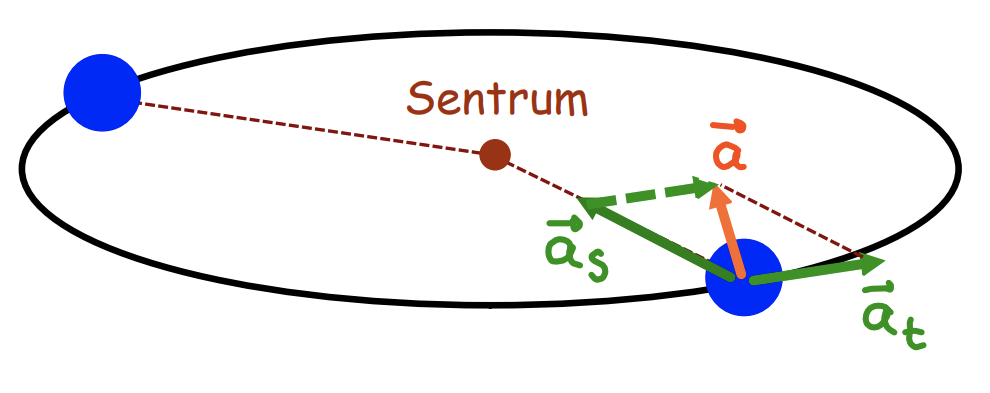
\includegraphics[width=10cm]{images/circle.png}
    \caption{Krefter ved variabel banefart}
\end{figure}


$a_s \bot a_t$

\begin{itemize}
    \item[] \textbf{Vektorsum:} $\Vec{a} = \Vec{a_s} + \Vec{a_t}$
    \item[] \textbf{Størrelse:} $|\Vec{a}| = \sqrt{a_s^2+a_t^2}$
    \item[] \textbf{Retning:} $tan (\alpha) = \frac{a_s}{a_t}$
\end{itemize}

    

\subsection{Pendelbevegelser}
\subsubsection{Med snordrag}
$S-G \cdot cos\theta = m\frac{v^2}{r}$


\section{Luftmotstand}
\subsection{Lav fart}
Strømlinjene krysser ikke hverandre.
Luftmotstanden er en friksjonskraft mellom legemet og lufta!\\
$f = kv$
\pagebreak
\subsection{Høy fart ($v \geq 10km/t $)}
Strømlinjene er kaotiske.\\
$f = kv^2$

\bigskip
$$k = \frac{1}{2}\rho AC_d\cdot v^2$$
\textbf{Konstanten $k$ sier noe om:}
\begin{itemize}
    \item[-] Legemets form
    \item[-] Luftas/væskens massetetthet $\rho$
    \item[-] Dragkoeffesienten %C_d%
\end{itemize}

\section{Væskemotstand}
For a spherical object falling in a medium, the drag force is:
$$F_s = 6\pi r\eta v$$
\begin{itemize}
    \item[] $r =$ objektets radius
    \item[] $\eta =$ mediumets viskositet
    \item[] $v =$ objektest hastighet gjenom mediumet
\end{itemize}

\section{Arbeid og Energi}
\subsection{Mekanisk arbeid}
\subsubsection{Konstant kraft}
Det mekaniske arbeider utført av den konstante krafta $\Vec{F}$ over en forflytning $\Delta\Vec{s}$ er definert ved skalarproduktet:
$$W = \Vec{F} \cdot \Delta\Vec{s} = F_x \cdot \Delta s = F \cdot cos\theta \cdot\Delta s$$
%
\subsubsection{Variabel kraft}
\textbf{Triks i ludo:} se på en svært liten forflytning $\Delta x$. Da er kraften tilnærmet konstant.
Det totale mekaniske arbeidet mellom posisjon $x_1$ og $x_2$ er gitt ved summen av integralet:
$$W = \int_{x_1}^{x_2} dW = \int_{x_1}^{x_2} s(x) dx $$
%
\subsection{Effekt}
\subsubsection{Grunnleggende definisjon:} 
Effekt: $\frac{\text{Utført mekanisk arbeid}}{\text{Tid}}$
$$P = \frac{dW}{dt} = \Rightarrow \frac{J}{s} = Watt$$

\subsubsection{Mer generell definisjon}
$$P = \frac{dW}{dt} = \frac{\Vec{F}\cdot d\Vec{s}}{dt} = \Vec{F}\cdot\frac{ d\Vec{s}}{dt} = \Vec{F}\cdot\Vec{v} = F\cdot v\cdot cos \theta$$
$$\downarrow$$
$$P = F\cdot v\cdot cos \theta$$
%
\subsection{Kinetisk energi}
Kinetisk energi er en \underline{\textbf{skalar størrelse}} og har \underline{\textbf{ingen retning}}:
$$K = \frac{1}{2}mv^2$$

Endringen i et legemes kinetiske energi tilsvarer det mekaniske arbeidet utført på dette legemet:
$$W = \frac{1}{2}mv^2 - \frac{1}{2}mv_0^2 = \Delta K$$
\subsection{Potensiell energi}
$$U = mgh$$

\section{Energibevaring}
Energi kan ta svært mange ulike former
\begin{itemize}
    \item[-] \textbf{Potensiell energi} (opplagret energi i et legeme/system)
    \item[-] \textbf{Kinetisk energi} (bevegelsesenergien til et legeme/system)
    \item[-] \textbf{Varme} (oppstår ved at friksjonskrefter virker)
\end{itemize}
\subsubsection{}
\textbf{Energibevarlingsloven: }$\frac{1}{2}mv_0^2+mgh_0 = \frac{1}{2}mv^2+mgh$
$$W = \Delta K = -\Delta U$$

\section{Impuls og støt}
\subsection{Bevegelsesmengde (massefart)}
Moment = bevegelsesmengde (massefart)\\
$$\Vec{p} = m\Vec{v}$$\\
Momentet har en retning!
\subsubsection{Bevaring av det totalet momentet}
\begin{itemize}
    \item[-] Dersom legemet kun påvirkes av \underline{\textbf{indre krefter}} er det totalet momentet \textbf{bevart}. Slike systemer kalles \textbf{"Lukkede systemer"}
    $$\Vec{P}_{\text{før}} = \Vec{P}_{\text{etter}} $$
    $$\Updownarrow$$
    $$M\Vec{v} = m_1\Vec{v}_1 + m_2\Vec{v}_2 + \dots + m_n\Vec{v}_n$$
    \item[-] Dersom legemet påvirkes av \underline{\textbf{ytre krefter}} er det totalet momentet \textbf{ikke bevart}. Disse kreftene vil nemlig  endre farten(e) underveis og dermed størrelsen(e) $m\Vec{v}$.
\end{itemize}

\pagebreak
\subsection{Impuls}
Impulsen som virker på et legeme er gitt ved at en kraft $\Vec{F}$ virker på et legeme over et tidsrom $\Delta t$
$$\Vec{F}\cdot \Delta t$$
Impulsen endrer ballens fart. $\Rightarrow$ veggen virker med en kraft som endrer $\Vec{v}$

\subsubsection{\textbf{Impulsloven:}}
\begin{figure} [H]
    \centering
    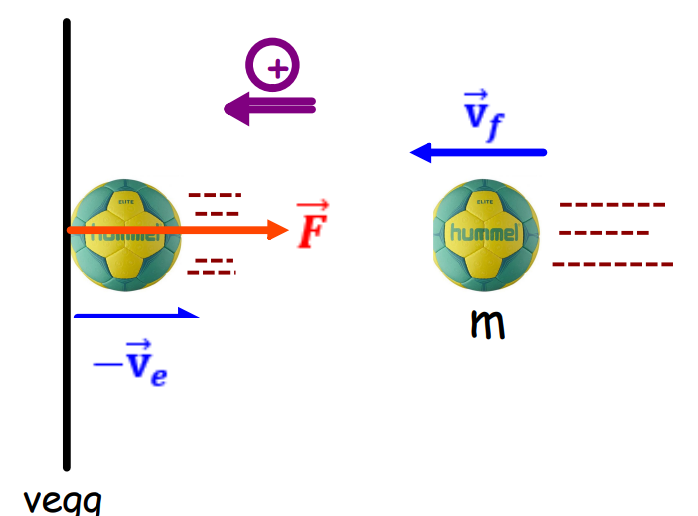
\includegraphics[height=4cm]{images/impuls.png}
    \caption{Impulsloven}
\end{figure}
En konstants kraft $\Vec{F}$ gir en impuls:
$$\Vec{F} = m\Vec{a} = m\frac{\Delta\Vec{v}}{\Delta t} \Rightarrow \Vec{F}\cdot\Delta t = m\cdot\Delta\Vec{v} = m(\Vec{v_{etter}} - \Vec{v_{før}})$$
Håndballens momentvektor $\Vec{p}$ endrer seg som en konsekvens av at krafta virker på den.
Håndballens momentvektor endres som en konsekvens av at \underline{fartsvektoren endrer retning.}\\
\bigskip
\color{blue}
Merk deg at ballens masse $m$ og hastighet $|\Vec{v}| = v$ \underline{ikke} trenger å endre verdi!
\color{black}
\pagebreak
\subsubsection{Vektoriell beskrivelse av impulsloven}
\begin{figure} [H]
    \centering
    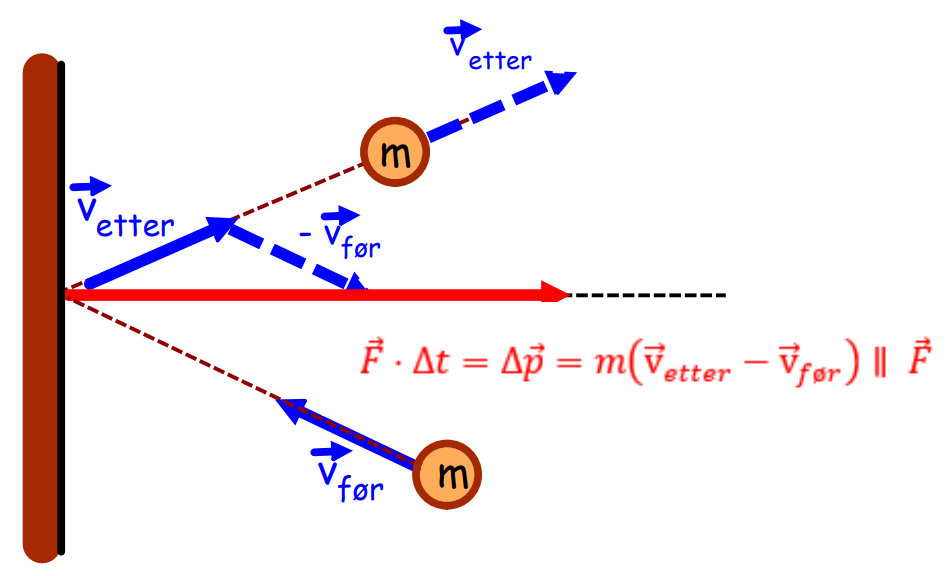
\includegraphics[height = 4cm]{images/impuls2.png}
    \caption{Ikke-paralelle fartsvektorer}
\end{figure}
\begin{figure} [H]
    
    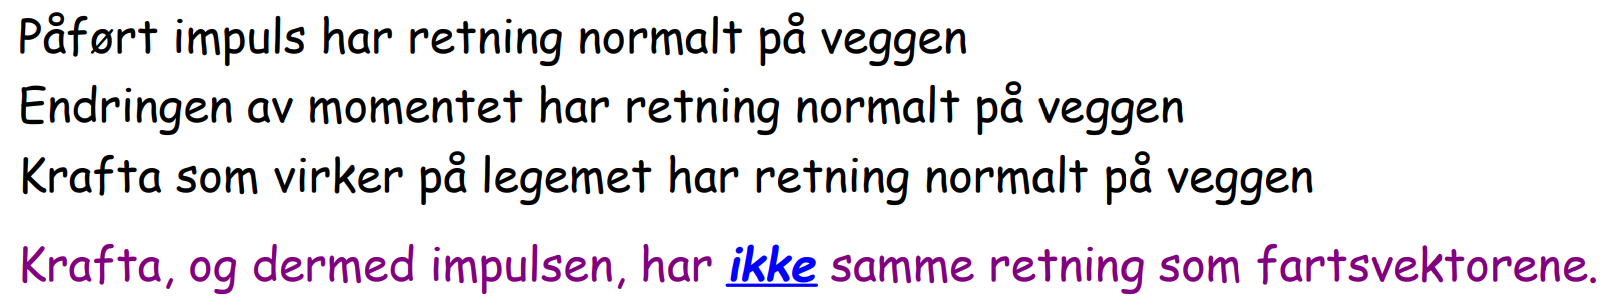
\includegraphics[width=14cm]{images/impuls-text.png}
\end{figure}

$$\Vec{F}\cdot \Delta t = \Delta \Vec{p} = m(\Vec{v_{etter}} - \Vec{v_{før}})$$


\subsection{Støtprosesser}
\bigskip
\subsubsection{1. Uelastiske støt}
Energi går \textbf{tapt}:\\
- Friksjonsvarme (oppvarming)\\
- Legemene deformeres\\
\bigskip
\textbf{Momentet er bevart} før og etter støtprosessen. Kun indre krefter virker i kollisjonsøyeblikket.\\
\bigskip
Den kinetiske energien er \textbf{ikke bevart} etter støtprosessen som en direkte konsekvens av energitapet antydet over.\\
\bigskip
 Kan deles i to undergrupper: \\
 \textbf{Uelastiske støt:} legemene henger ikke sammen etter sammenstøtet.\\
 \textbf{Fullstendig uelastiske støt:} legemene henger sammen etter sammenstøtet\\
 \bigskip
\subsubsection{2. Fullstendig elastiske støt}
Ugreie å regne på da vi får en ekstra bevegelsesligning.\\
Eksempel på fullstendig elastisk støt: støt mellom biljardkuler.

Legemene henger \textbf{ikke sammen} etter sammenstøtet.\\
\bigskip
Energi går \textbf{ikke tapt}:\\
- Friksjonsvarmen til omgivelsene er neglisjerbar\\
- Legemene deformeres ikke\\
\bigskip
\textbf{Momentet er bevart} før og etter støtprosessen. Kun indre krefter virker i kollisjonsøyeblikket.\\
\bigskip
Den kinetiske energien er \textbf{ikke bevart} etter støtprosessen som en direkte konsekvens av at energitapet er neglisjerbart.\\
\bigskip

\section{Rakettfremdrift}
Raketten brenner drivstoff(masse), og akselerer underveis.\\
\bigskip
Formel for skyvekraften:\\
$v =$ startfarten\\
$m =$ masse\\
$dm =$ masse drivstoff brent\\
$u =$ eksosgass hastighet\\

$$\Vec{u}\frac{dm}{dt} = -m\frac{dv}{dt} = -\Vec{F}_{skyv}$$

Formel for rakettfremdrift:
$$v-v_0 = u\cdot ln(\frac{m_0}{m})$$

\section{Massesenter}
\subsection{Kraftmoment}
Definisjon på kraftmoment/dreiemoment: $\tau = Kraft \cdot arm = F\cdot r$\\
Du anvender en kraft $F$ for å rotere et legeme i forhold til en rotasjonsakse(hengslene).

Dersom oppgaven spør om vinkler:
\begin{figure} [H]
    \centering
    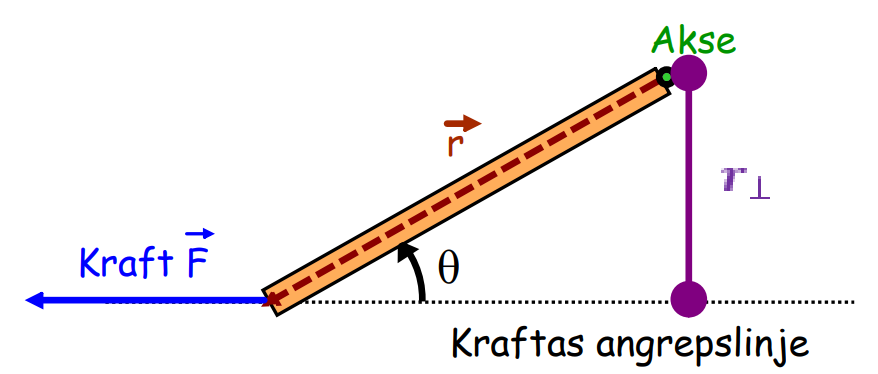
\includegraphics[height = 4cm]{images/torque.png}
    \caption{Kraftmoment}
\end{figure}
$$\tau = |\Vec{r}\cdot \Vec{F}| = r\cdot F \cdot sin\theta = F\cdot r_{\perp}$$

\subsection{Massefordeling}
Den totale massen til et legeme kan være \textbf{diskret(på ett punkt)} fordelt eller \textbf{kontinuerlig(langs en linje)} fordelt. 

\subsubsection{Diskret massefordeling. 1 dimensjon}
$$CM = \frac{m_1x_1+m_2x_2}{m_1+m_2} = \frac{1}{M}(m_1x_1+m_2x_2) = \frac{1}{M}\sum_i{m_ix_i}$$
$M = m_1+m_2$

\subsubsection{Kontinuerlig massefordeling. 1 dimensjon}
F.eks. sylinder(sugerør)

Masse pr. lengdeenhet gitt ved: $\lambda = \frac{dm}{dx}$\\
Massesenter (CM): $\Bar{x} = \frac{1}{M} \int x dm$

\subsubsection{Diskret massefordeling 2 dimensjoner}
$$\Vec{r}_{CM} = (\Bar{x}, \Bar{y}) = \left[ \frac{1}{M} \sum_i x_im_i, \frac{1}{M} \sum_i y_i m_i \right]$$

\subsubsection{Kontinuerlig massefordeling. 2 dimensjoner}
$$dm = \sigma dA = \sigma dxdy$$
Massesenter (CM):
$$\Vec{r}_{CM} = (\Bar{x}, \Bar{y}])= \left[\frac{1}{M} \iint x_i dm, \frac{1}{M} \iint y_idm\right]$$

der eksempelvis
$$\iint x_i dm = \iint x_i \sigma dxdy = \sigma \int x_idx\cdot \int dy$$

\subsubsection{Diskret massefordeling 3 dimensjoner}
$$\Vec{r}_{CM} = (\Bar{x}, \Bar{y}, \Bar{z}) = \left[\frac{1}{M} \sum_i x_im_i, \frac{1}{M} \sum_i y_i m_i, \frac{1}{M} \sum_i z_i m_i \right]$$

\subsubsection{Kontinuerlig massefordeling. 3 dimensjoner}
$$dm = \rho dV = \rho dxdydz$$
Massesenter (CM):
$$\Vec{r}_{CM} = [\Bar{x}, \Bar{y}, \Bar{z}] = \left[\frac{1}{M} \iiint x_i dm, \frac{1}{M} \iiint y_idm, \frac{1}{M} \iiint z_idm \right]$$

der eksempelvis
$$\iiint x_i dm = \iiint x_i \rho dV = \rho \int x_i dx\cdot \int dy \cdot \int dz$$

\newpage
\section{Rotasjonsmekanikk}
\subsection{Treghetsmoment}
Finner treghetsmomentet $I$ ved å slå opp i tabell.
\begin{figure} [H]
    \centering
    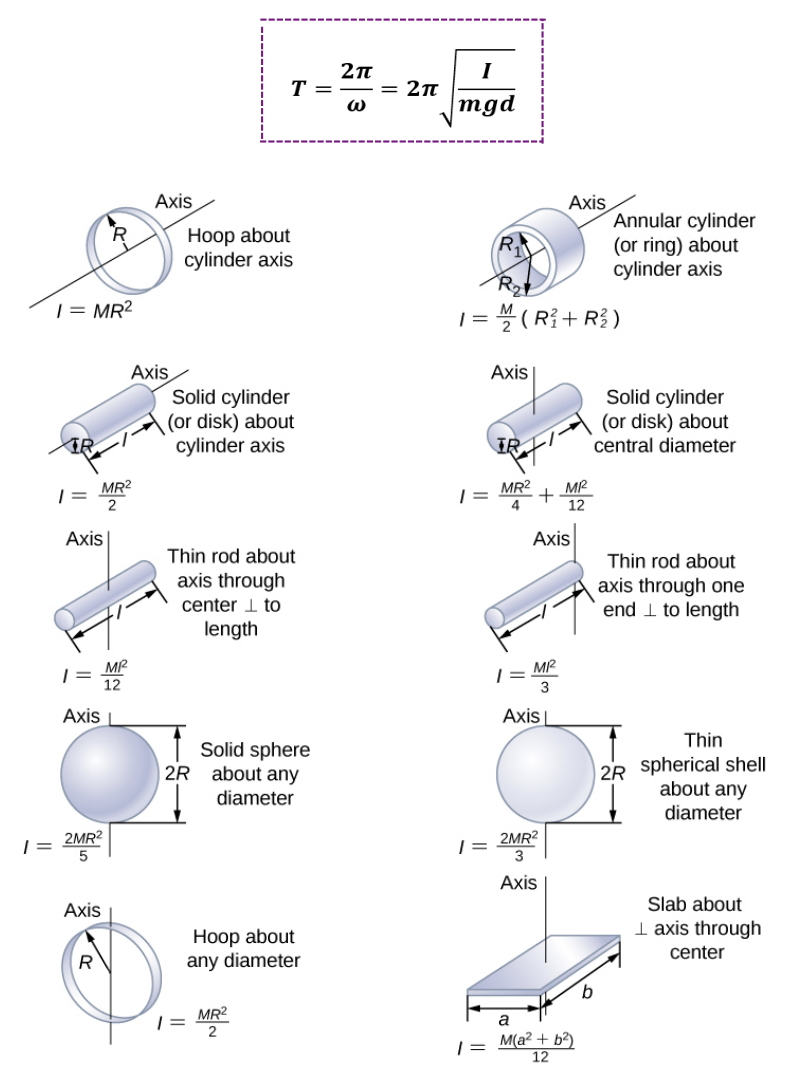
\includegraphics[width = 6cm]{images/slow.png}
    \caption{Tabell for treghetsmoment}
\end{figure}
\subsubsection{Steiners sats/paralellakseteoremet}
Steiners sats brukes til å beregne treghetsmomentet $i$ til et legeme som ikke har massesenter på rotasjonsaksen.
\begin{figure} [H]
    \centering
    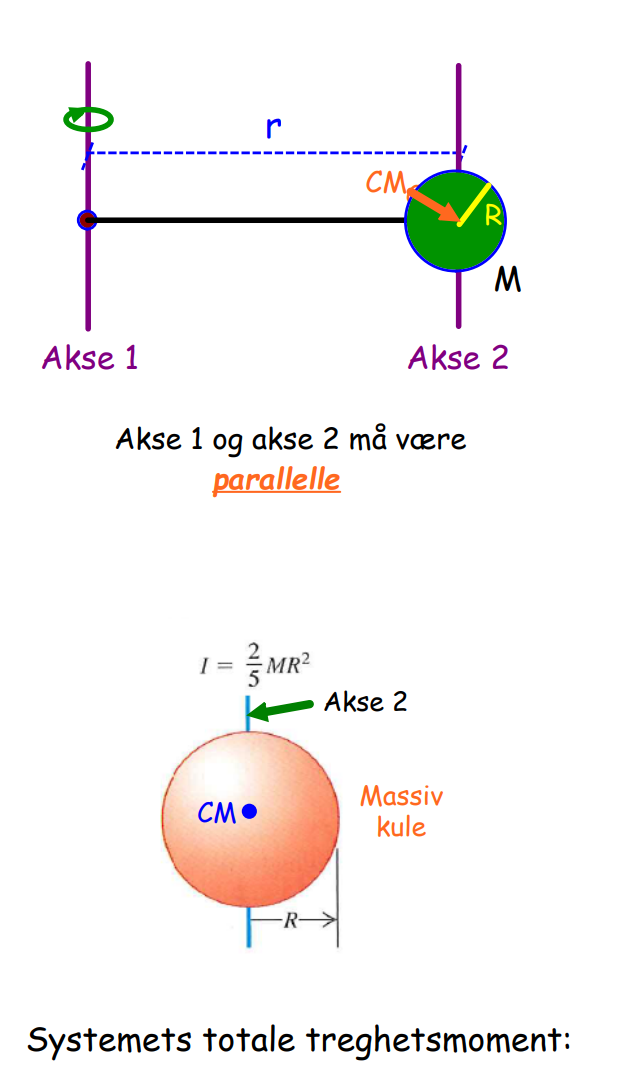
\includegraphics[height = 10cm]{images/steiner.png}
    \caption{Steiners sats}
\end{figure}
$$I_{tot} = I_k + I_{CM} = \frac{2}{5}MR^2+Mr^2$$

\underline{\textbf{Helt generelt:}}\\
Steiners sats brukes til å beregne det totale treghetsmomentet til et legeme om en vilkårlig akse (akse 1) som er parallell med en akse (akse 2) som går gjennom legemets massesenter (CM).
$$I_{tot} = I_0 + Md^2$$
\begin{figure} [H]
    \centering
    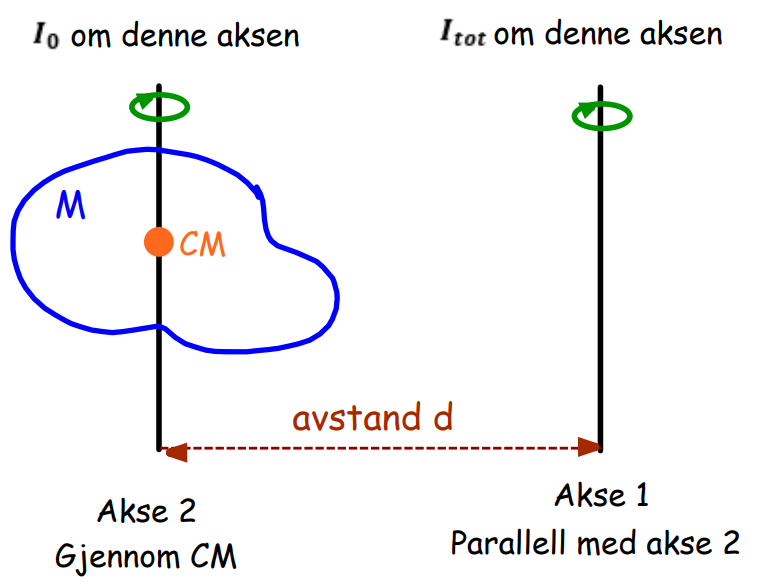
\includegraphics[height = 5cm]{images/steiner2.png}
    \caption{Steiners sats generelt}
\end{figure}


\subsection{Newtons 2. lov på rotasjonsform}
$$\sum \tau_t = I\cdot \alpha$$
$\alpha =$ vinkelakselerasjon\\
Merk: sentripetalakselerasjonen bidrar \textbf{ikke} til å endre legemets banehastighet.


\subsection{Rotasjonskinetiske energien}
\begin{figure} [H]
    \centering
    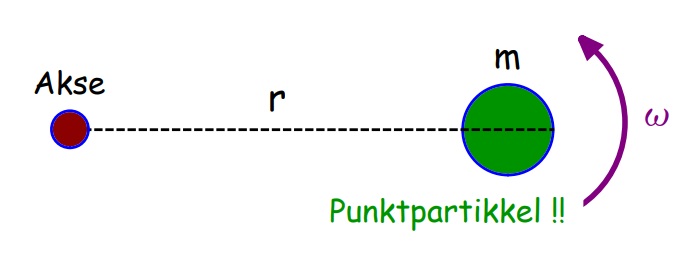
\includegraphics[height = 4cm]{images/rotation_kinetic.png}
    \caption{Rotasjonskinetiske energien}
\end{figure}
$$K = \frac{1}{2}(mr^2)\omega^2 = \frac{1}{2}I\omega^2$$
Den rotasjonskinetiske energien \underline{\textbf{varierer}}:
\begin{enumerate}
    \item Ene og alene når avstanden $r$ ut fra rotasjonsaksen varierer. det vil si: hvor langt ut fra aksen punktpartikkelen befinner seg. Vinkelhastigheten $\omega$ kan være konstant.
    \item Ene og alene dersom massen $m$ endrer seg. Dette er i analogi med det lineære tilfellet.
\end{enumerate}

\subsection{Arbeid of effekt ved rotasjon}
I det lineære tilfellet fant vi formelen $p = F\cdot v$ for effekten $p$.
For en rotasjonsbevegelse blir formelen:
$$P = \tau \cdot \omega$$

\subsection{Rullende bevegelser}
\subsubsection{Kastebevegelse}

\begin{figure} [H]
    \centering
    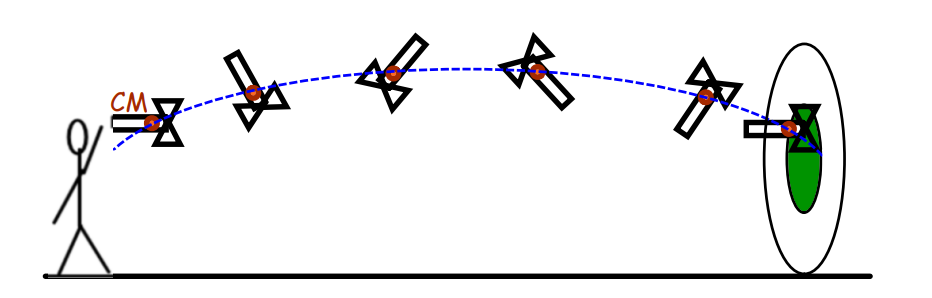
\includegraphics[height = 4cm]{images/throw.png}
    \caption{Kastebevegelse}
\end{figure}
\textbf{Bevegelsen er satt sammen av to deler:}
\begin{enumerate}
    \item \underline{Translasjon av massesenteret:}\\
    Beskrivelsen av bevegelsesligningene for kastebevegelse.\\
    Massesenteret følger en \underline{\textbf{parabelbane}}.\\
    Newtons 2. lov: $\sum F = ma_{CM}$

    \item \underline{Rotasjonsbevegelse omkring massesenteret:}\\
    Beskrives av Newtons 2. lov på rotasjonsform: $\sum \tau = I\alpha$\\
    $I =$ treghetmomentet om aksen som går gjennom CM
\end{enumerate}
\textbf{Bevegelsesformlene for kastebevegelse med rotasjon:}
\begin{itemize}
    \item[] $s_{x,CM} = v_{x,CM}\cdot t$
    \item[] $v_{y,CM} = v_{0y,CM} + a_{CM}t$
    \item[] $S_{y,CM} = \frac{v_{y,CM}+v_{0y,CM}}{2}\cdot t$
    \item[] $s_{y,CM} = v_{0y,CM}\cdot t + \frac{1}{2}a_{CM}t^2$
    \item[] $V^2_{7,CM} - v^2_{0y,CM} = 2a_{CM}s_{y,CM}$
\end{itemize}

\subsection{Den totale kinetiske energien ved kombinert lineær- og rotasjonsbevegelse}
\begin{figure} [H]
    \centering
    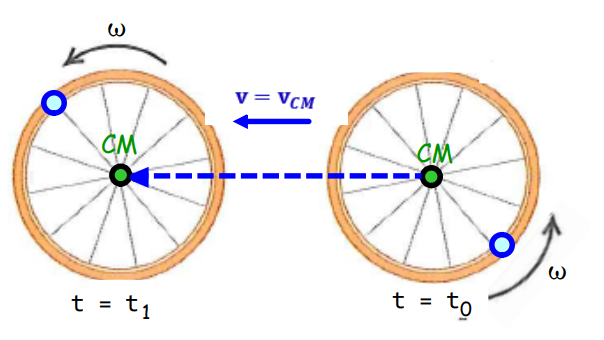
\includegraphics[height = 4cm]{images/roll.png}
    \caption{Rulling}
\end{figure}
Figruen viser et elgeme der massesenteret ($CM$) forflytter seg lineært rett samtidig som at alle masse-element roterer omkring dette massesenteret.\\
Den totale kinetiske energien for dette rullende hjulet, som stadig beveger seg lineært bortover er gitt ved:
$$E_K = \frac{1}{2}mv^2_{CM}+\frac{1}{2}I\omega^2$$
\begin{itemize}
    \item[] Første leddet, $\frac{1}{2}mv^2_{CM}$, står for den lineære hastigheten.\\
    \item[] Andre leddet, $\frac{1}{2}I\omega^2$, står for rotasjonshastigheten.
\end{itemize}

\subsection{Rulling uten sluring}
$$v_{CM} = \frac{2\pi}{\Delta t} \cdot r = \omega r$$

\subsection{Dreieimpuls}
Eksempel på dreieimpuls: håndball som treffer åpen dør. Døren begynner å rotere.

\begin{figure} [H]
    \centering
    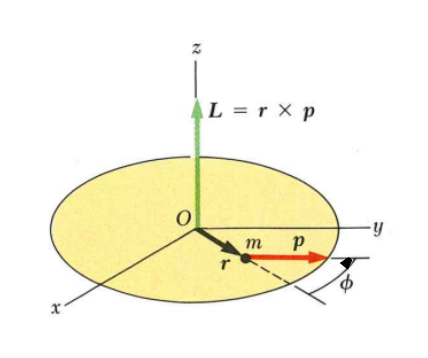
\includegraphics[height = 4cm]{images/dreieimpuls.png}
    \caption{Dreieimpuls}
\end{figure}
$$\Vec{L} = \Vec{r} \times \Vec{p} = \Vec{r} \times m\Vec{m} = m\Vec{r} \times \Vec{m}$$
Retningen til $\Vec{L}$ er angitt av \textbf{høyrehåndsregelen}:
\begin{itemize}
    \item[] $\Vec{L}$ peker oppover: roterer \underline{\textbf{mot}} klokka
    \item[] $\Vec{L}$ peker nedover: roterer \underline{\textbf{med}} klokka
\end{itemize}
\subsubsection{Størrelsen til banedreieimpulsen til partikkelen/legemet:}
$$L = m(r_{\perp}\cdot v) = mr_{\perp}v$$
$L = kgm^2/s$\\
Legemets dreieimpuls er konstant i \underline{alle posisjoner} langs sirkelbanen.

\subsubsection{Dreieimpulsens påvirkning av dreiemmoment}
Hva skjer med dreieimpulsen $L$ dersom vi påvirker legemet med et dreiemoment $\rho$?\\
Banehastigheten $v = r\omega$ endrer seg! Da endrer også dreieimpulsen seg ettersom den er gitt ved $L = mr_\perp \textbf{v}$\\

$$\Delta L = I\cdot\Delta \omega = \tau \cdot \Delta t$$
Spinnsatsen: $\frac{\Delta L}{\Delta t} = \sum \tau \Rightarrow \sum \tau\cdot\Delta t = \Delta L$\\
\bigskip
Impulsloven i det lineære: $F\cdot \Delta t = \Delta p$

\subsubsection{Bevarelse av dreieimpuls}
Dersom det ikke virker et dreiemoment på et objekt, er dreieimpulsen bevart.\\
En kunstløper vil snurre raskere dersom hun tar inn armene ($r$ minker), men dreieimpulsen er bevart.

\section{Mekaniske Svingninger}
\subsection{Harmoniske svingninger}
Finner diff. likning ved å bruke hooks lov:
\begin{itemize}
    \item[] $F = -kx = ma$
    \item[] $\Rightarrow a = \frac{d^2x}{dt^2} = -\frac{k}{m}x$
    \item[] $\Rightarrow \frac{d^2x}{dt^2}-\omega_0^2x \Leftrightarrow \omega_0 = \sqrt{\frac{k}{m}} = $ konstant
\end{itemize}
\begin{figure} [H]
    \centering
    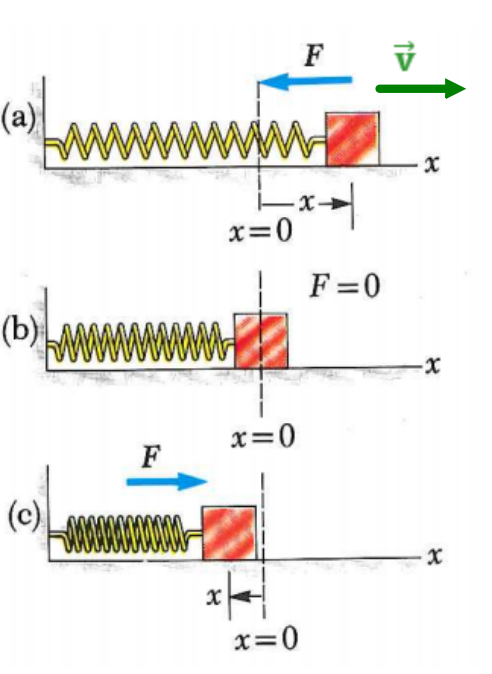
\includegraphics[height = 4cm]{images/swing.png}
    \caption{Harmoniske svingninger}
\end{figure}
Klossens svingefunksjon:
$$x(t) = a\cdot cos(\omega_0t) + b\cdot sin(\omega_0t)$$
$$\Rightarrow R \cdot cos(\omega_0t - \Phi)$$
\bigskip
\subsubsection{Perioden T}
Tiden $T$ det tar å  fullføre $2\pi$ radianer = en hel svingning.
$$\omega_ot = \omega_0T = 2\pi \Rightarrow T = \frac{2\pi}{\omega_0} = 2\pi \sqrt{\frac{m}{k}}$$


\subsubsection{Frekvens $f$}
Frekvensen $f$ angir hvor mange hele svinginger som klossen i figur 11 fullfører per sekund.
$$f = \frac{1}{T} = \frac{\omega_o}{2\pi} = \frac{1}{2\pi}\sqrt{\frac{k}{m}} \Rightarrow \omega_0 = 2\pi f$$



\subsubsection{Forskjell mellom svingefrekvens $\omega_o$ og vinkelhastighet $\omega$}
\textbf{Vinkelhastighet $\omega$:}\\
Vinkelhastigheten til denne pendelen, som svinger harmonisk fram og tilbake, er gitt ved:
$$\omega(t) = \frac{d\theta}{dt} = \omega_1 + \alpha t = \frac{v_1}{R} + \frac{a}{R}t = \frac{1}{R}(v_1+at) = \frac{v(t)}{R}$$
Vinkelhastigheten $\omega$ \underline{\textbf{varierer}} under svingningen ettersom banehastigheten $v$ varierer.\\
\begin{figure} [H]
    \centering
    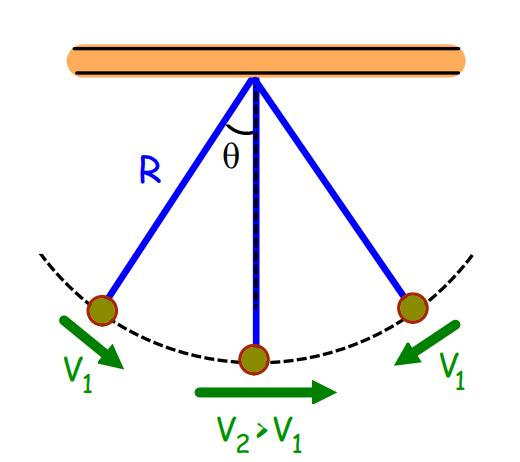
\includegraphics[height = 4cm]{images/pendel.png}
    \caption{Vinkelhastighet $\omega$}
\end{figure}
\bigskip
\textbf{Svingefrekvens}\\
Svingefrekvensen $\omega_0 = \sqrt{\frac{k}{m}}$ = \underline{konstant}.\\
$\omega_0$ angir at klossen (figur 11) fullfører et konstant antall radianer ila. et bestemt tidsrom $t$.

\subsection{Mekaniske pendler}
\subsubsection{Den oscillerende pendelen}
\begin{figure} [H]
    \centering
    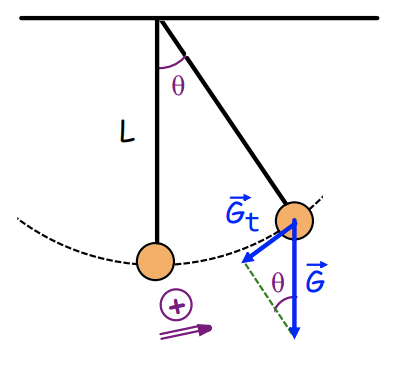
\includegraphics[height = 4cm]{images/pendel2.png}
    \caption{Oscillerende pendel}
\end{figure}

Pendelen svinger på grunn av gravtiasjonskraften.
\begin{itemize}
    \item[] Svingefrekvens: $\omega_0 = \sqrt{\frac{g}{L}}$
    \item[] Periode: $T = \frac{2\pi}{\omega_0} = 2\pi\sqrt{\frac{L}{g}}$
\end{itemize}

\subsubsection{Den fysiske pendelen}
\begin{figure} [H]
    \centering
    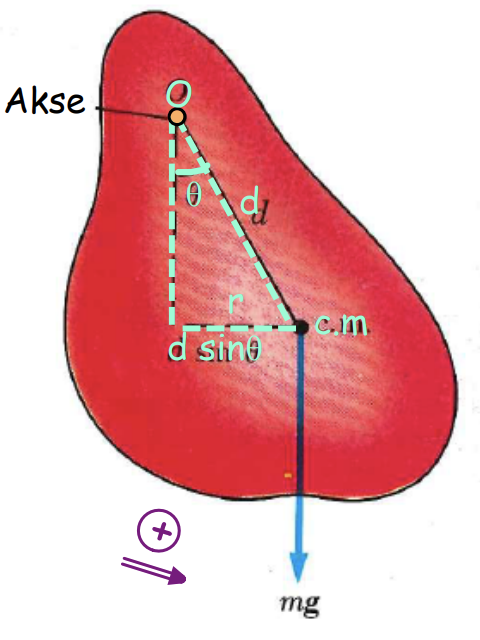
\includegraphics[height = 4cm]{images/physicalPendel.png}
    \caption{Fysisk pendel}
\end{figure}
Treghetsmomentet $I$ driver svingningen.
\begin{itemize}
    \item[] Svingefrekvens: $\omega_0 = \sqrt{\frac{mgd}{I}}$
    \item[] Periode: $T = \frac{2\pi}{\omega_0} = 2\pi\sqrt{\frac{I}{mgd}}$
\end{itemize}
\subsubsection{Torsjonspendelen}
\begin{figure} [H]
    \centering
    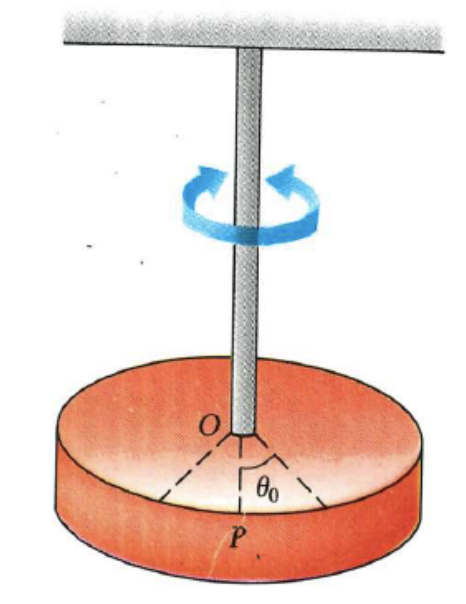
\includegraphics[height = 4cm]{images/tortion.png}
    \caption{Torsjonspendel}
\end{figure}
En torsjonspendel roterer fram og tilbake om sitt eget sentrum der snora er festet, uten av snora krøller seg.\\
\bigskip
Hooks lov på rotasjonsform: $\tau = -k\theta$\\
\bigskip
Merk deg at skivas forflytning nå er en vinkelforflytning $\theta$. Dreiemomentet $\tau$ sier noe om snoras evne til å produsere en svingebevegelse/rotasjonsbevegelse.

\begin{itemize}
    \item[] Svingefrekvens: $\omega_0 = \sqrt{\frac{K}{I}}$
    \item[] Periode: $T = \frac{2\pi}{\omega_0} = 2\pi\sqrt{\frac{I}{K}}$
\end{itemize}


\subsubsection{Sammenlikning pendler}
\begin{figure} [H]
    \centering
    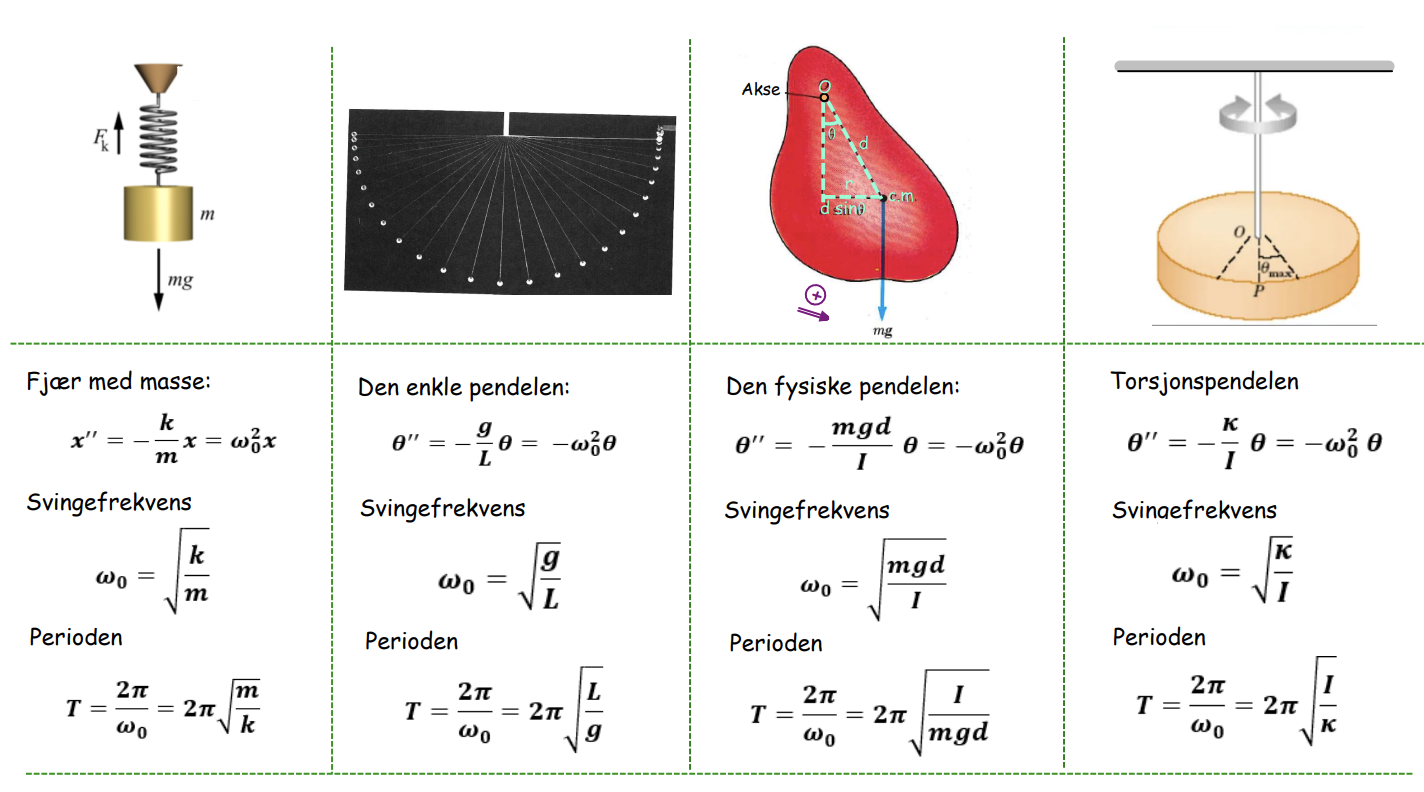
\includegraphics[width = 13.5cm]{images/comparison.png}
    \caption{Sammenlikning pendel}
\end{figure}

\subsection{Dempede svingninger med fjær}
\begin{figure} [H]
    \centering
    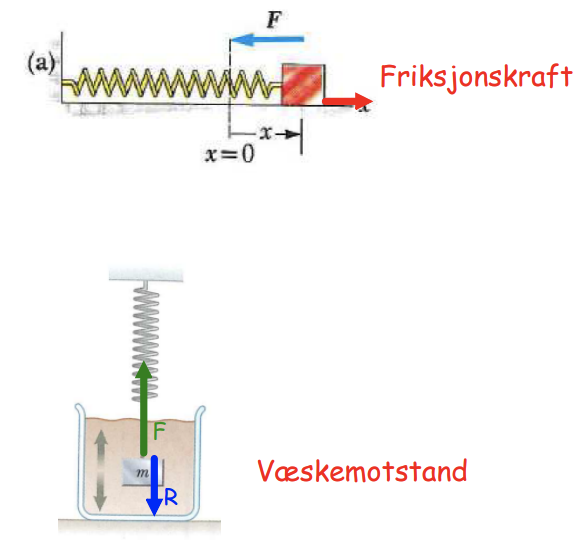
\includegraphics[width = 10cm]{images/dempede.png}
    \caption{Dempede svingninger}
\end{figure}
Det virker en friksjonskraft mellom kloss og materialet klossen er i kontakt med.
$$md''+bx'+kx=0$$
\underline{3 ulike løsninger:}
\begin{enumerate}
    \item Overdemping: $1-\frac{4mk}{b^2} > 0$
    \item Kritisk demping: $1-\frac{4mk}{b^2} = 0$ (Reell løsning)
    \item Demped svingning $1-\frac{4mk}{b^2} < 0$ (Komplekse løsninger)
\end{enumerate}
\subsubsection{Overdemping}
Kjennetegnet på et overdempet system: $4mk < b^2$
$$x(t) = e^{r_1t} + e^{r_2t}; \hspace{5em} r_{1,2} = \frac{b}{2m}\left(-1 \pm \sqrt{1-\frac{4mk}{b^2}}\right)$$
$r_1 < 0$ og $r_2 < 0$\\
Dette vil si at $x(t)$ er ekspotensielt avtagende:
\begin{figure} [H]
    \centering
    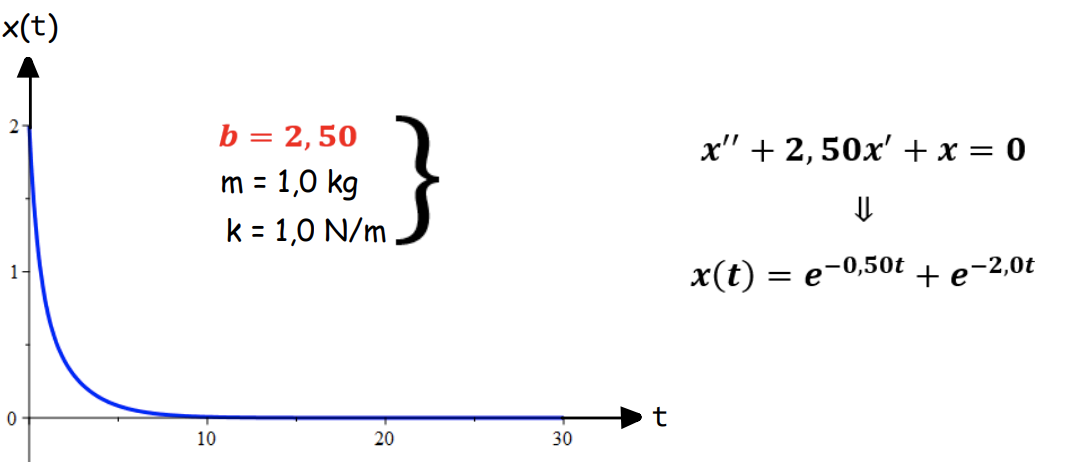
\includegraphics[width = 8cm]{images/slow1.png}
    \caption{x(t)}
\end{figure}

\subsubsection{Kritisk demping}
Kjennetegn på et kritisk system: $4mk = b^2$
$$x(t) = e^{rt} + te^{rt}; \hspace{5em} r = -\frac{b}{2m} < 0$$

Dette vil si at $x(t)$ er ekspotensielt avtagende:
\begin{figure} [H]
    \centering
    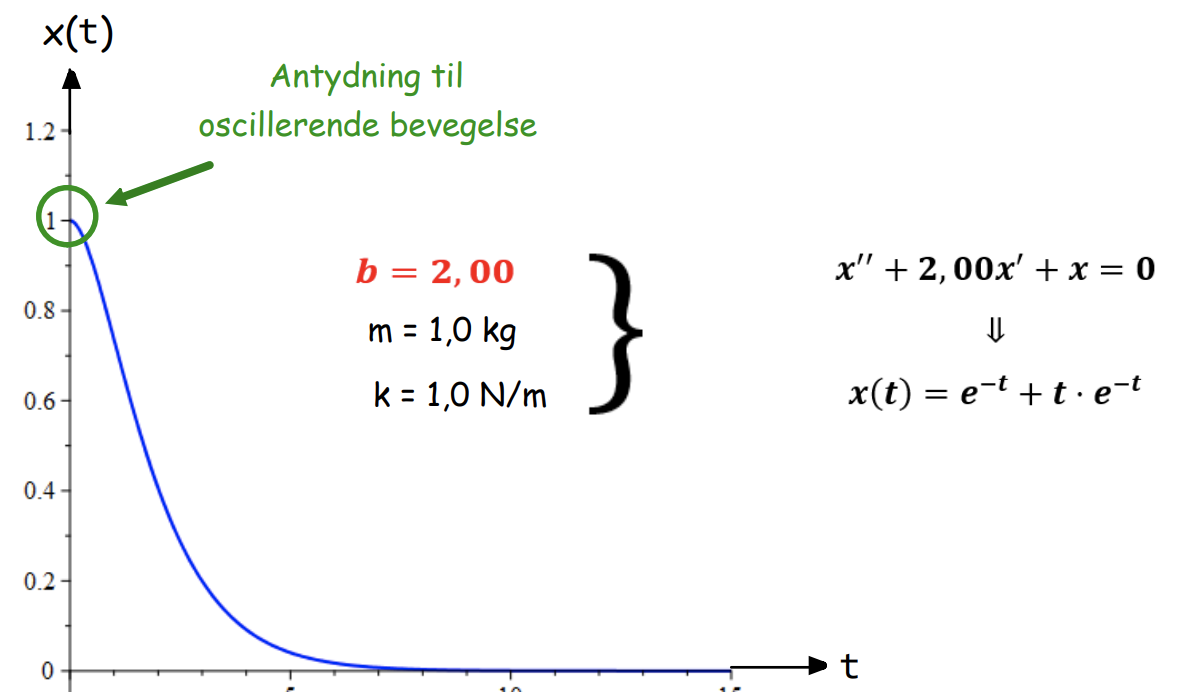
\includegraphics[width = 8cm]{images/slow2.png}
    \caption{x(t)}
\end{figure}

\subsubsection{Dempet svingning}
Kjennetegn på et kritisk system: $4mk > b^2$
$$x(t) = \sqrt{2}e^{-\frac{b}{2m}t} cos \left( \frac{\sqrt{b^2-4mk}}{2m}t-\phi  \right)$$
Amplituden $A$ avtar med tiden $t$: $\sqrt{2}e^{-\frac{b}{2m}t}$\\
- Svingningen \underline{dempes} raskere med økende dempningskoeffisienten $b$\\
- Amplituden \underline{avtar} raskere med økende dempningskoeffesient $b$
- Svingefrekvensen: $\omega = \frac{\sqrt{b^2-4mk}}{2m}$ = konstant\\
Dette vil si at $x(t)$ er periodisk avtagende:
\begin{figure} [H]
    \centering
    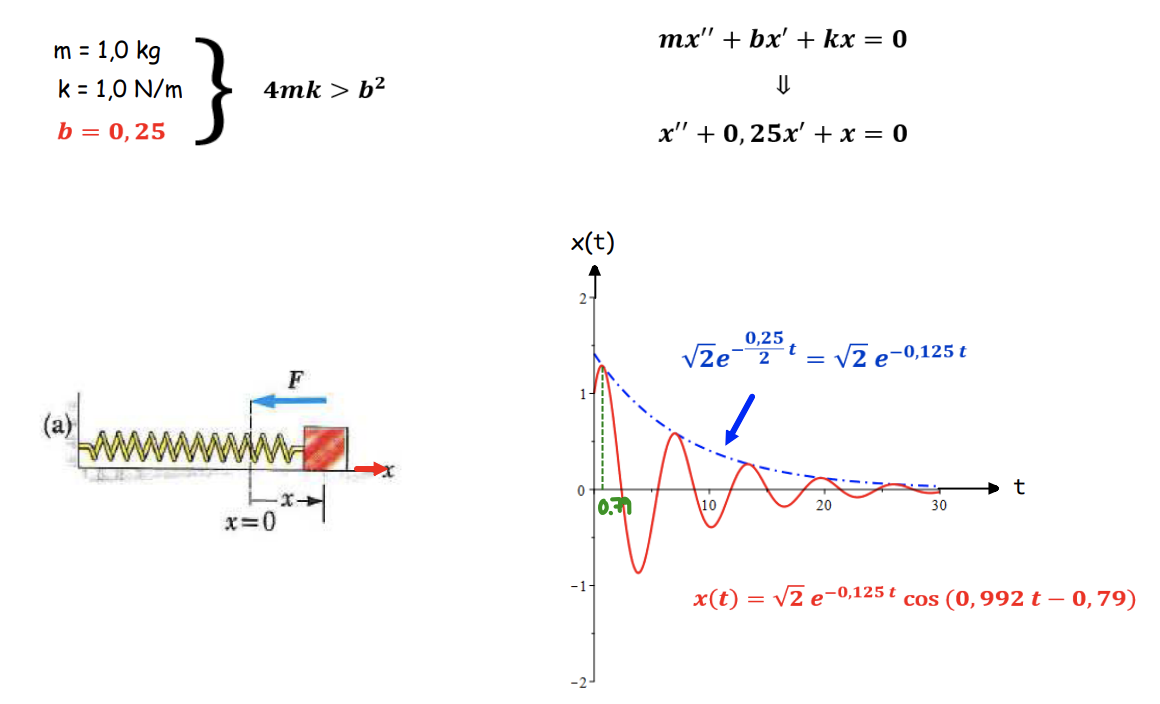
\includegraphics[width = 8cm]{images/slow3.png}
    \caption{x(t)}
\end{figure}
\bigskip
\textbf{\underline{Kvasifrekvensen $\mu$}}\\
\bigskip
$\omega = \frac{\sqrt{b^2-4mk}}{2m}$= konstant der $4mk > b^2$\\
Rent matematisk representerer dette en kompleks svingefrekvens. Komplekse svingefrekvenser har ingen mening i en praktisk setting. Det har reelle frekvenser!\\
\bigskip
Vi innfører derfor en \underline{kvasifrekvens} der vi tar absoluttverdien av uttrykket inne i rota:
$$\mu = \frac{\sqrt{|b^2-mk|}}{2m} = \frac{\sqrt{mk-b^2}}{2m}$$
$$\mu = \left(1-\frac{b^2}{8mk}\cdot \omega_0 \right)$$
Svingefrekvensen avtar med økende dempingsfaktor b, og er maksimal for en harmonisk oscilliator.
\begin{figure} [H]
    \centering
    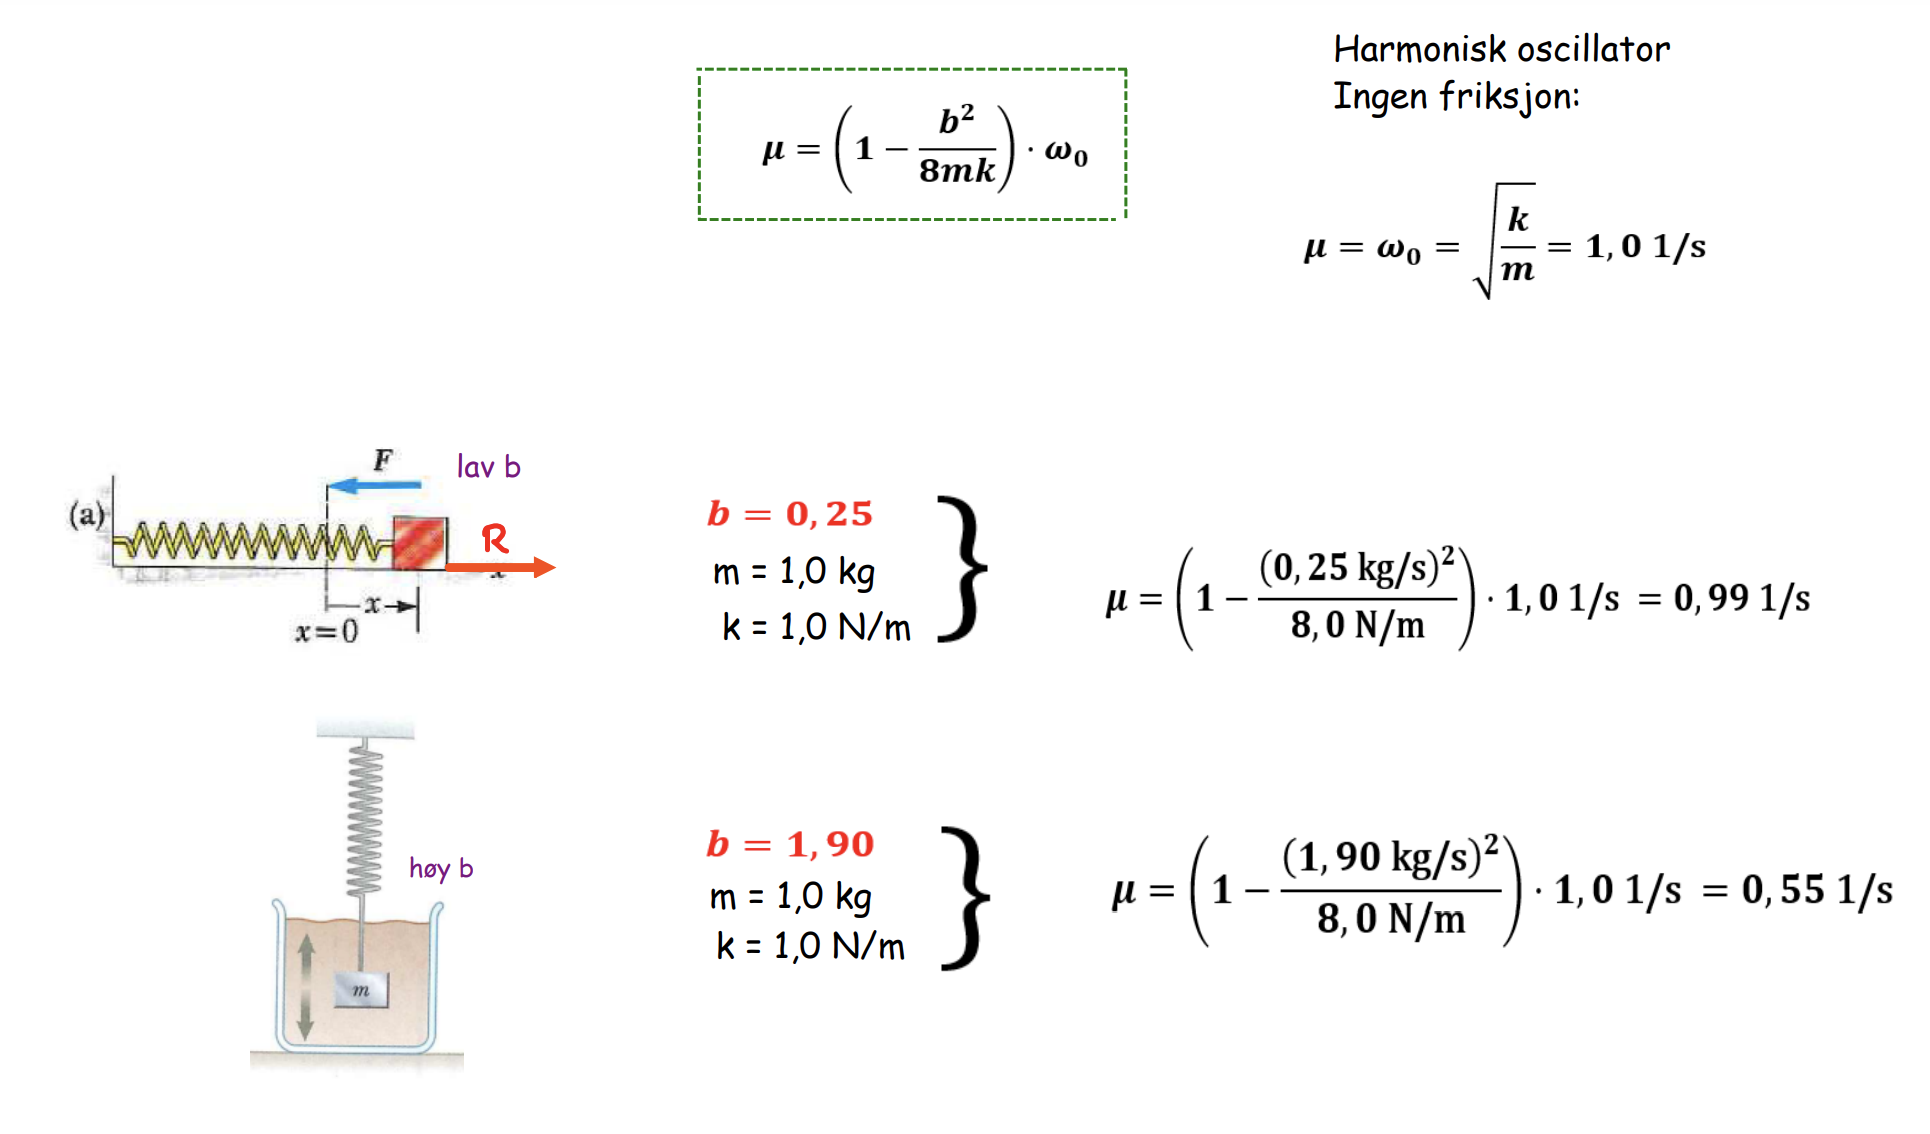
\includegraphics[width = 10cm]{images/slow4.png}
    \caption{Kvasifrekvens}
\end{figure}
\pagebreak
\section{Bølger}
\subsection{Bølgeforplanting langs en streng}
\begin{figure} [H]
    \centering
    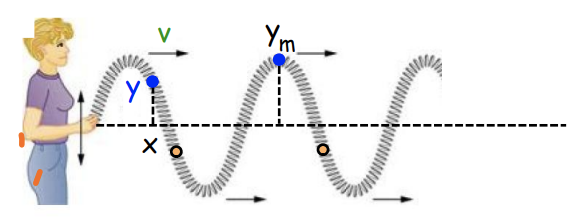
\includegraphics[width = 8cm]{images/waves.png}
    \caption{Kvasifrekvens}
\end{figure}
Bølgen forplanter seg med konstant hastighet v.
Generell bølgefunksjon:
$$y(x,t) = A sin(kx-\omega t + \phi)$$
\begin{itemize}
    \item[-] $A$ angir amplituden til bølgen.
    \item[-] $\omega = 2\pi v$: Vinkelfrekvens
    \item[-] Bølgetallet $k = \frac{2\pi}{\lambda}$: antall bølger per periode $2 \pi$. 
    \item[-] $t$ angir den tiden en bølgebruker på å forplante seg langs strengen.
    \item[-] $\phi$: fasekonstanten
    \item[-] $y$ angir den den vertikale forflytningen av en vilkårlig del av strengen på et vilkårlig tidspunkt $t$
\end{itemize}
$\lambda = \frac{v}{f} \Rightarrow$ Desto kortere bølgelengde $\lambda$, desto høyere frekvens (konstant $v$)\\
Desto høyere bølgetallet $k$ er, desto høyere er bølgens svingefrekven $\omega$. $\omega_0 = k\cdot v$

\subsection{Fasehastigheter og energitransport}
\begin{figure} [H]
    \centering
    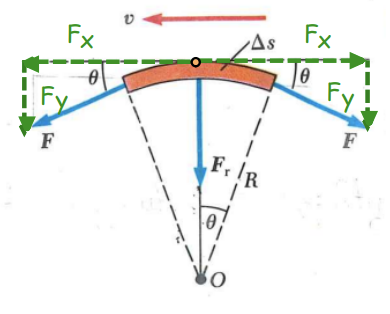
\includegraphics[width = 6cm]{images/wavy.png}
    \caption{Bølgefart}
\end{figure}
\begin{itemize}
    \item[] Kreftene som virker i x-retning: $\sum F = 0$
    \item[] Kreftene som virker i y-retning: $F_y = Fsin(\theta) \Rightarrow \sum F_y = 2Fsin(\theta) = 2F\theta$ for en liten $\theta$
    \item[] Massen $m$ til masseelementet $\Delta s$: $m = \mu \cdot \Delta s = 2\pi R\theta = \frac{\Delta m}{\Delta x}$. ($\mu$ = materialkonstant)
    \item[] Sentripetalkraft: $F_r = m \frac{v^2}{R}$
    \item[] Forplantningshastigheten $v$: $v = \sqrt{\frac{F}{\mu}}$. $F =$ strekkrafta, $\mu =$ massetettheten til strengen. Avhengig av strammheten til strengen, massetettheten til strengen. \underline{\textbf{Ikke}} avhengig av frekvensen $f$.  Massetetthet kan også oppgis som $\rho = kg/m^3 $ og $\sigma = kg/m^2 $.
    \item[] Total energi $E_T$: $E_T = \frac{1}{2}\mu\Delta x \omega_0^2A^2$
    \item[] Effekten $p$: $p = E_T \cdot v$

Ved konvertering fra f.eks. $\rho$ til $\mu$ må man gange med arealet (tverrsnittet) til kabelen.
\end{itemize}
\subsubsection{Energitransport langs en streng}
\begin{figure} [H]
    \centering
    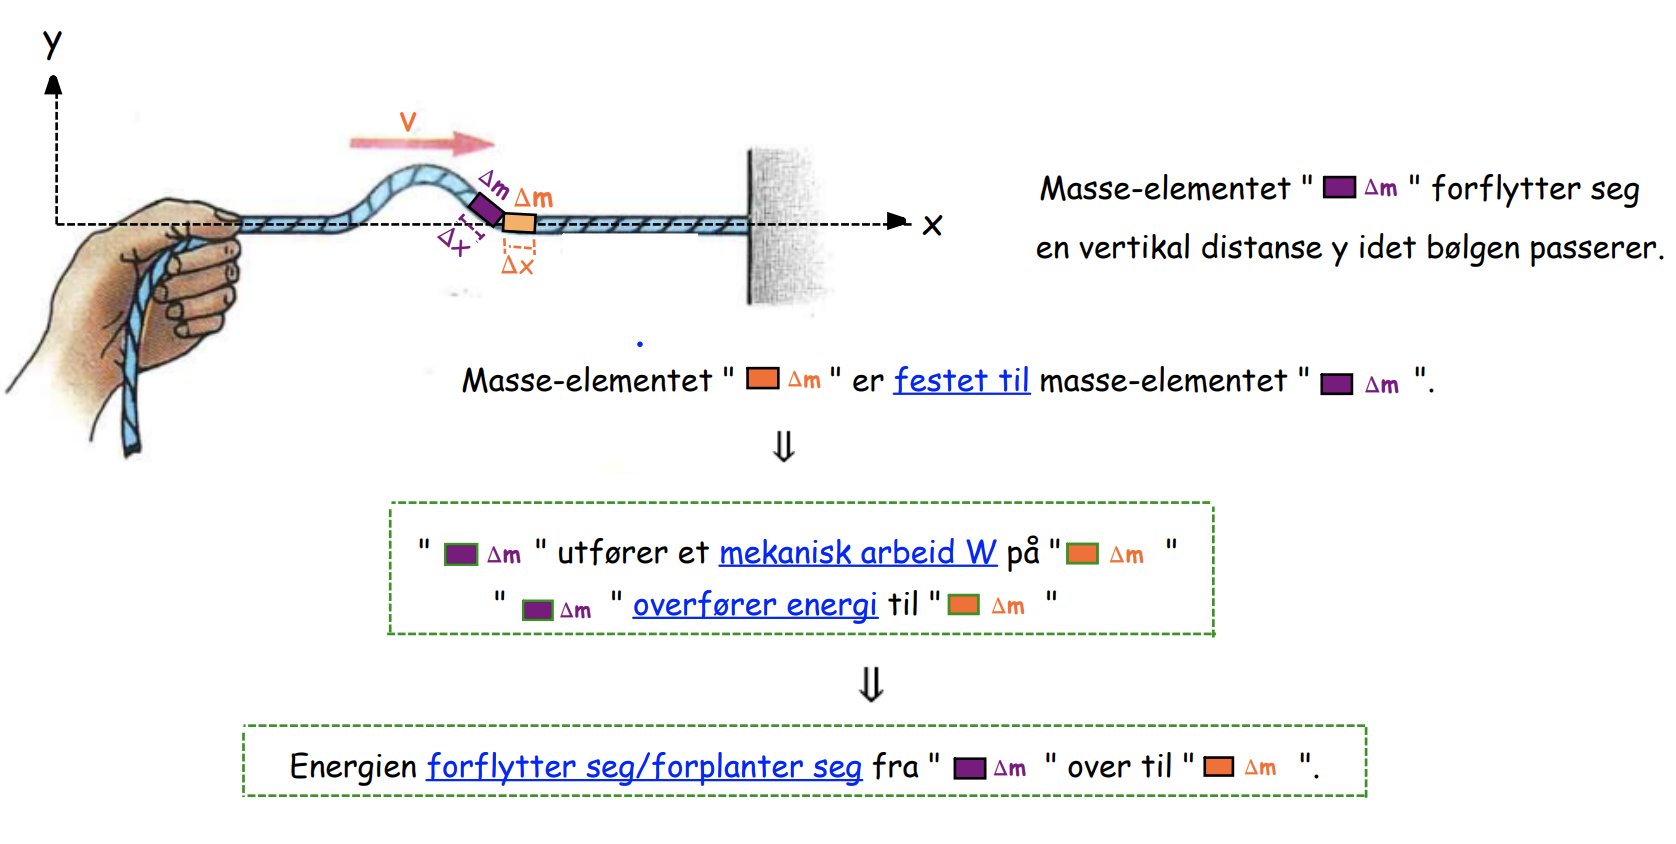
\includegraphics[width = 13cm]{images/string.png}
    \caption{Energitransport langs en streng}
\end{figure}

Bølgehastigheten er konstant! Kreftene på begge sider av bølgen strammer opp strengen.\\
For et masseelement på strengen:
\begin{itemize}
    \item[] $\Delta s \approx$ sirkelbue med radius $R$
    \item[] Masse elementet erfarer en sentripetalkraft $F_r$
    \item[] Sentripetalakselerasjon: $a_r = \frac{v^2}{R}$
\end{itemize}

\subsection{Resonans}
\subsubsection{Interferens}
\textbf{Interferens}: amplituden til to bølger som møtes legges sammen. $A_r = A_1+ A_2$\\
Kan være konstruktiv og destruktiv.\\

\subsubsection{Stående bølger}
For at en stående bølge skal oppstå må vi ha:
\begin{itemize}
    \item[-] Samme amplitude $A$
    \item[-] Samme svingefrekvens $\omega$
    \item[-] Samme bølgelengde $\lambda$
\end{itemize}
Bølgene må videre:
\begin{itemize}
    \item[-] Interferere
    \item[-] Forplante seg langs samme verdier
    \item[-] Forplante seg i motsatt retning i forhold til hverandre
\end{itemize}
\textbf{\underline{Matematikken:}}\\
\bigskip
To enkeltbølger:\\
$y_1 = A_0sin(kx-\omega t)$\\
$y_2 = A_0 sin(kx+\omega t)$\\
$k = \frac{2\pi}{\lambda}$\\
\bigskip
Den stående bølgen blir da:
$$y = y_1+y_2 = A_0sin(kx-\omega t) +  A_0 sin(kx+\omega t)$$
$$\Updownarrow$$
$$y = (2A_sin(kx)\cdot cos(\omega t)$$
\begin{itemize}
    \item [-] $(2A_sin(kx)$ beskriver den vertikale harmoniske svingningen gitt i enhver posisjon x langs x-aksen
    \item [-] $cos(\omega t))$ beskriver hvor lang tid $t$ det tar å fullføre en hel harmonisk svingning ($t=1$)
\end{itemize}

Vi kan finne maksimal amplitude ved å sette $A = 1$ og regne ut for $x$.\\
Vi kan finne nodene (punktet mellom bølgene som står i ro) ved å finne $x$ for $(2A_sin(kx) = 0$. $x = n\cdot \frac{\lambda}{2}$

\subsubsection{Refleksjon og transmisjon}
Newtons 3. lov! \underline{\textbf{Kraft = motkraft}}
\begin{figure} [H]
    \centering
    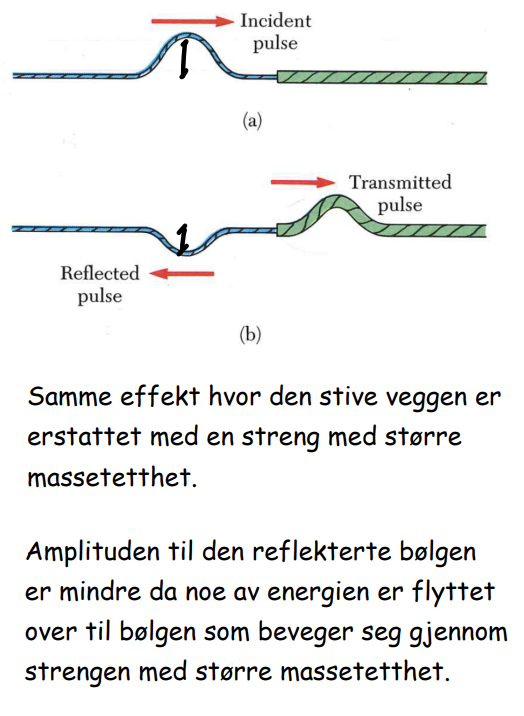
\includegraphics[width = 5cm]{images/bounce.png}
    \caption{Kraft = motkraft}
\end{figure}

\subsubsection{Resonans}
Generell formel:
$$x(t) =  c_1cos(\omega_0 t) + c_2cos(\omega_0 t) + \frac{F_0}{2m\omega_0}t\cdot sin(\omega_0t)$$
\begin{itemize}
    \item[] $c_1cos(\omega_0 t) + c_2cos(\omega_0 t)$ beskriver systemets indre svingning før den ytre krafta virker. Harmonisk svingning.
    \item[] $\frac{F_0}{2m\omega_0}t\cdot sin(\omega_0t)$ beskriver hvordan den ytre krafta $F_0$ påvirker det svingende systemets egen svingefrekvens (egenfrekvensen $\omega$) slik at amplituden øker. Den ytre krafta tilfører systemet energi.
\end{itemize}
\begin{figure} [H]
    \centering
    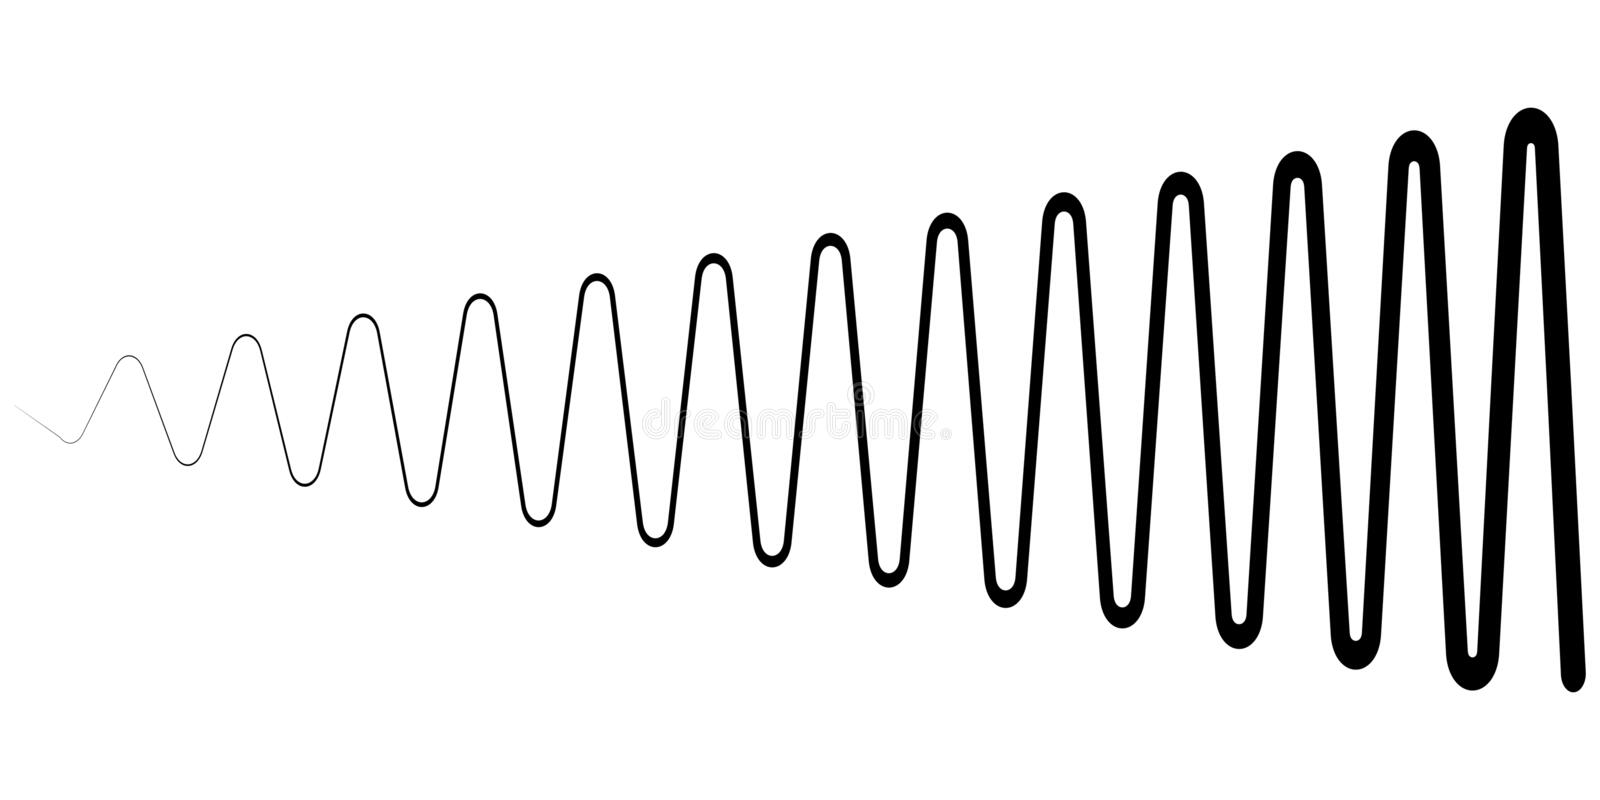
\includegraphics[width = 5cm]{images/resonans.jpg}
    \caption{Konstruktiv resonans}
\end{figure}
Vi kan ha både konstruktiv og destruktiv resonans.

\subsection{Lydhastigheter}
$$f = \frac{1}{T} = \frac{v}{\lambda}$$
I et gitt medium er lydhastigheten $v$ \underline{\textbf{konstant}}

\subsubsection{Lydhastigheter i ulike medium}
$$v=\sqrt{\frac{B}{S}} = \sqrt{\frac{B}{p}}$$
\begin{itemize}
    \item[] Bulkmodulen $B$ beskriver hvor mye volumet til et medium endres når det virker krefter fra alle kanter. Trykket: $p = \frac{F}{A}$ 
    \item[] $S$ = massetettheten
\end{itemize}
$$B = -\Delta p\cdot \frac{v}{\Delta v}$$
\begin{itemize}
    \item [] Stor $B \Rightarrow$ Liten volumendring
    \item [] Liten $B \Rightarrow$ Stor volumendring
\end{itemize}
\subsubsection{Harmoniske trykkbølger}
\begin{figure} [H]
    \centering
    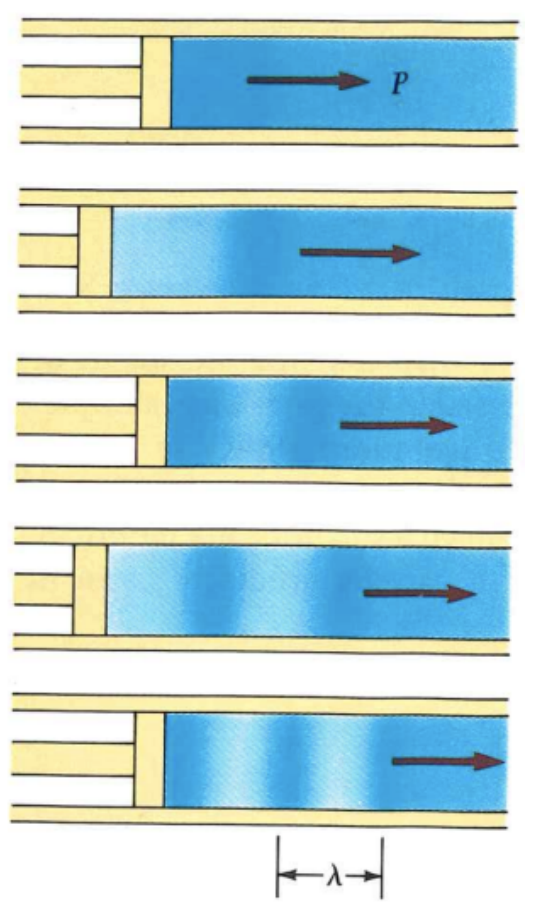
\includegraphics[width = 5cm]{images/compress.png}
    \caption{Harmoniske trykkbølger}
\end{figure}
Trykkendring:
$$\Delta p = -\delta v^2\frac{A\Delta S}{A\Delta x} = \delta v^2 S_m k sin (kx-\omega t) = \delta\cdot v\omega s_m sin(kx-\omega t)$$


\subsubsection{Intensiteten til en trykkbølge}
Intensiteten $I$ til en trykkbølge er et mål på hvor mye energi per tidsenhet (energitetthet). Det vil si $P$ som treffer en gitt arealflate $A$.

$$I_m = \frac{P}{A} = \frac{1}{2}\delta\omega^2s_m^2\cdot v$$
\begin{itemize}
    \item [] $\delta$: høyere $\delta \Rightarrow$ høyere $I$ 
    \item [] $\omega$: høyere $\omega \Rightarrow$ høyere $I$ 
    \item [] $s_m$: lav stemme vs. høy stemme. Mao. mediets sammentrekning/utvidelse. 
    \item [] $v$: hastigheten på bølgen som treffer flaten.
\end{itemize}
Maksimal intensitet uttrykt ved trykkendringen $\Delta p$:
$$I_m = \frac{1}{2}\delta\omega^2s_m^2\cdot v = \frac{1}{2}(\delta\omega s_m\cdot v)^2\cdot\frac{1}{\delta v} = \frac{\Delta P_m^2}{2\delta v}$$

\subsubsection{Lydnivå målt i desibel}
$$\beta = 10 log(\frac{I}{I_o})$$
\underline{\textbf{Laveste verdi}}\\
\bigskip
Laveste desibelverdi: Referanseverdi\\
Laveste intensitet: $I = I_0 = 10^{-12 w/m^2}$
$$\beta = 10 log(\frac{I_0}{I_0}) = 10 log 1 = 0dB$$

\underline{\textbf{Høyeste verdi}}\\
\bigskip
Høyeste intensitet: $I = 1,0 w/m^2$
$$\beta = 10 log(\frac{I}{I_0}) = 10 log(\frac{1,0}{10^{-12}}) = 10 log 10^{12} = 10\cdot 12 = 120dB$$

\subsection{Doppler effekten}
Doppler effekten beskriver hvordan en frekvensen av lyd-/lysbølge er avhengig relativt til hvordan observatøren/kilden beveger seg i forhold til hverandre. 
\begin{figure} [H]
    \centering
    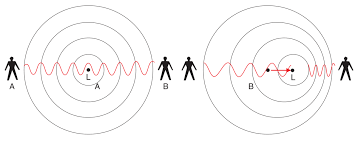
\includegraphics[width = 8cm]{images/doppler.png}
    \caption{Dopplereffekten}
\end{figure}
\begin{figure} [H]
    \centering
    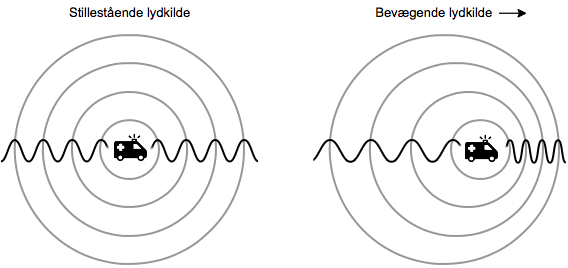
\includegraphics[width = 8cm]{images/doppler2.png}
    \caption{Dopplereffekten}
\end{figure}
$$f' = f\cdot (\frac{v+v_0}{v}) = f\cdot (1+\frac{v_0}{v}$$
Desto raskere du beveger deg mot de inkommende lydbølgene, desto flere bølgefronter rekker frem til deg ila. $t=1.0s$ og desto høyere frekvens $f'$ vil du registrere, og motsatt.

\underline{\textbf{Lydkilden beveger seg mot deg}}:
$$\lambda' = \frac{v}{f}-\frac{v_s}{f} = \lambda-\Delta\lambda; \hspace{5em \Delta\lambda = \frac{v_s}{f}}$$
- $\Delta \lambda =$ "reduksjonen" av lydbølgens reelle bølgelengde $\lambda$ som en direkte konsekvens av lydkildens hastighet $v_s$.

$$f' = \frac{v}{\lambda'} = \frac{v}{\frac{v}{f}-\frac{v_s}{f}} = f\cdot (\frac{v}{v-v_s}) = f\cdot \frac{1}{1-\frac{v_s}{v}}$$
- Desto raskere lydkilden kommer mot deg, desto høyere blir frekvensen $f'$, og desto "kortere" blir bølgelengden $\lambda$.\\
\bigskip
\bigskip
\underline{\textbf{Lydkilden beveger seg fra deg}}:
$$\lambda' = \frac{v}{f}-\frac{v_s}{f} = \lambda +\Delta\lambda; \hspace{5em \Delta\lambda = \frac{v_s}{f}}$$

$$f' = \frac{v}{\lambda'} = \frac{v}{\frac{v}{f}+\frac{v_s}{f}} = f\cdot (\frac{v}{v+v_s}) = f\cdot \frac{1}{1+\frac{v_s}{v}}$$
- Desto raskere lydkilden beveger seg fra deg, desto lavere blir frekvensen $f'$, og desto lengre blir bølgelengden $\lambda$.


\end{document}
